\documentclass[
  xcolor={svgnames}, 
  hyperref={citecolor=DeepPink4,linkcolor=DarkRed,urlcolor=DarkBlue},
  %handout
]{beamer}
%% Packages
\usepackage{amssymb}
\usepackage{amsmath}
\usepackage{amsthm}
\usepackage{amsfonts}
\usepackage{mathtools}
\usepackage{xspace}
\usepackage{bm}
\usepackage{nicefrac}
\usepackage{bbm}
\usepackage{boxedminipage}
\usepackage{xparse}
\usepackage[x11names]{xcolor}
\usepackage{float}
\usepackage{multirow}
\usepackage{graphicx}
\usepackage{caption}
\usepackage{subcaption}
\usepackage{ifthen}
\usepackage{algpseudocode}
%\usepackage{algorithmic}
\usepackage{array}
\usepackage{wrapfig}
\usepackage{geometry}
%\usepackage{enumitem}
\usepackage{pgfplots}


\usepackage{tikz}
\usetikzlibrary{positioning}
\usetikzlibrary{fit}
\usetikzlibrary{calc}
\usetikzlibrary{backgrounds}
\usetikzlibrary{shapes}
\usetikzlibrary{patterns}
\usetikzlibrary{matrix}
\usetikzlibrary{intersections}

\usepackage[pdftex,bookmarks=true,pdfstartview=FitH,colorlinks,linkcolor=blue,filecolor=blue,citecolor=blue,urlcolor=blue,pagebackref=true]{hyperref}
    \urlstyle{sf}
    
% No figures taking up one whole page
\renewcommand{\floatpagefraction}{.8}%

%% Document Design Choices
%\setlength{\parindent}{0pt}
%\setlength{\parskip}{10pt}
%\renewcommand{\labelitemi}{\ensuremath{\circ}}
\geometry{left=1in, right=1in, top=1in, bottom=1in}
\makeatletter
\renewcommand{\paragraph}{%
	\@startsection{paragraph}{4}%
	{\z@}{4pt \@plus 0pt \@minus 0pt}{-1em}%
	{\normalfont\normalsize\bfseries}%
}
\makeatother


%% Marking
\newcommand\TODO[1]{{\color{red}{#1}}\xspace}

%% Theorems and Environments
%
%\makeatletter
%\newtheorem*{rep@theorem}{\rep@title}
%\newcommand{\newreptheorem}[2]{%
%\newenvironment{rep#1}[1]{%
% \def\rep@title{\theoremref{##1} Restated}%
% \begin{rep@theorem}}%
% {\end{rep@theorem}}}
%\makeatother
%
%\makeatletter
%\newtheorem*{rep@lemma}{\rep@title}
%\newcommand{\newreplemma}[2] {%
%\newenvironment{rep#1}[1]{%
% \def\rep@title{\lemmaref{##1} Restated}%
% \begin{rep@lemma}}%
% {\end{rep@lemma}}}
%\makeatother
%
\newtheorem{theorem}{Theorem}
%\newreptheorem{theorem}{Theorem}
\newtheorem{importedlemma}{Imported Lemma}
\newtheorem{importedtheorem}{Imported Theorem} 
%\newtheorem{informaltheorem}{Informal Theorem}
\newtheorem{definition}{Definition}
\newtheorem{lemma}{Lemma}
\newtheorem{proposition}{Proposition}
%\newreplemma{lemma}{Lemma}
\newtheorem{claim}{Claim}
\newtheorem{corollary}[theorem]{Corollary}
\newtheorem{observation}{Observation}


\newenvironment{boxedalgo}
  {\begin{center}\begin{boxedminipage}{\linewidth}}
  {\end{boxedminipage}\end{center}}


%% References
\newcommand{\namedref}[2]{\hyperref[#2]{#1~\ref*{#2}}\xspace}
\newcommand{\lemmaref}[1]{\namedref{Lemma}{lem:#1}}
\newcommand{\propref}[1]{\namedref{Proposition}{prop:#1}}
\newcommand{\theoremref}[1]{\namedref{Theorem}{thm:#1}}
\newcommand{\claimref}[1]{\namedref{Claim}{clm:#1}}
\newcommand{\corolref}[1]{\namedref{Corollary}{corol:#1}}
\newcommand{\figureref}[1]{\namedref{Figure}{fig:#1}}
\newcommand{\tableref}[1]{\namedref{Table}{tbl:#1}}
\newcommand{\equationref}[1]{\namedref{Equation}{eq:#1}}
\newcommand{\defref}[1]{\namedref{Definition}{def:#1}}
\newcommand{\observationref}[1]{\namedref{Observation}{obs:#1}}
\newcommand{\procedureref}[1]{\namedref{Procedure}{proc:#1}}
\newcommand{\importedtheoremref}[1]{\namedref{Imported Theorem}{impthm:#1}}
\newcommand{\informaltheoremref}[1]{\namedref{Informal Theorem}{infthm:#1}}
\newcommand{\importedlemmaref}[1]{\namedref{Imported Lemma}{implem:#1}}

\newcommand{\sectionref}[1]{\namedref{Section}{sec:#1}}
\newcommand{\appendixref}[1]{\namedref{Appendix}{app:#1}}


%% English
\newcommand{\ie}{\text{i.e.}\xspace}
\newcommand{\st}{\text{s.t.}\xspace}
\newcommand{\etal}{\text{et al.}\xspace}
\newcommand{\naive}{\text{na\"ive}\xspace}
\newcommand{\wrt}{\text{w.r.t.}\xspace}
\newcommand{\whp}{\text{w.h.p.}\xspace}
\newcommand{\resp}{\text{resp.}\xspace}
\newcommand{\eg}{\text{e.g.}\xspace}
\newcommand{\cf}{\text{cf.}\xspace}
\newcommand{\visavis}{\text{vis-\`a-vis}\xspace}
\newcommand{\aka}{\text{a.k.a.}\xspace}


%% Names
\newcommand{\gacs}[0]{G\'acs\xspace}
\newcommand{\korner}[0]{K\"orner\xspace}
\newcommand{\turan}[0]{Tur{\'a}n\xspace}
\newcommand{\erdos}[0]{Erd\H{o}s\xspace}


%% Crypto
\def\alice{{{Alice}}\xspace}
\def\bob{{{Bob}}\xspace}
\def\eve{{{Eve}}\xspace}
%\newcommand{\poly}{\ensuremath{\mathrm{poly}}\xspace}
\DeclareMathOperator{\poly}{poly}
\DeclareMathOperator{\polylog}{polylog}
\newcommand{\negl}{\ensuremath{\mathsf{negl}}\xspace}
\newcommand{\secpar}{\ensuremath{{\kappa}}\xspace}
\newcommand{\zo}{\ensuremath{{\{0,1\}}}\xspace}

  %% Protocol Tree
  \def\Achildren{\mathsf{AliceChildren}}
  \def\Bchildren{\mathsf{BobChildren}}
  \def\Echildren{\mathsf{EveChildren}}
  
  %% Functionalities
  \newcommand{\func}[1]{\ensuremath{\cF_{\mathsf{#1}}}\xspace}
  \newcommand{\fcom}[0]{\func{com}}
  \newcommand{\fot}[0]{\func{ot}}
  
  %% Protocols
  % \newcommand{\prot}[1]{\ensuremath{\pi_{\mathsf{#1}}}\xspace}


%% Graph Theory
\newcommand{\ancest}[0]{\mathsf{Ancestors}}
\newcommand{\sibling}[0]{\mathsf{Siblings}}
\newcommand{\parent}[0]{\mathsf{parent}}
\newcommand{\leaves}[0]{\mathsf{leaves}}


%% Math Symbols
\renewcommand{\o}[0]{\ensuremath{\circ}\xspace}
\newcommand{\dist}[1]{\ensuremath{\left\langle{#1}\right\rangle}\xspace}
\newcommand{\prob}[2]{\ensuremath{\dist{{#1}_1, \dotsc, {#1}_{#2}}}\xspace}
\newcommand{\ip}[2]{\ensuremath{\left\langle{#1},{#2}\right\rangle}\xspace}
\renewcommand{\vec}[1]{\ensuremath{\mathbf{#1}}\xspace}
\newcommand{\concat}[0]{\ensuremath{\circ}\xspace}
\newcommand{\nin}[0]{\ensuremath{\not\in}\xspace}
\newcommand{\xor}[0]{\ensuremath{\oplus}\xspace}
\newcommand{\rv}[1]{\ensuremath{\mathbf{#1}}\xspace}
\newcommand{\p}[1]{\ensuremath{^{{\left(#1\right)}}}\xspace}
\newcommand{\argmax}[0]{\ensuremath{\mathop{\mathrm{argmax}}\;}\xspace}
\newcommand{\argmin}[0]{\ensuremath{\mathop{\mathrm{argmin}}\;}\xspace}
\newcommand{\maj}[0]{\ensuremath{\mathop{\mathrm{maj}}\;}\xspace}
\NewDocumentCommand\mathstack{>{\SplitList{;}}m}
  {\ensuremath{
    \begin{smallmatrix}
      \ProcessList{#1}{ \insertone }    
    \end{smallmatrix}
  }}
\newcommand{\insertone}[1]{\ensuremath{#1}\\}

%\newcommand{\argmax}{\operatornamewithlimits{argmax}}
%\DeclareMathOperator*{\argmax}{arg\,max}

  
  %% General
  \newcommand{\ceil}[1]{\ensuremath{\left\lceil{#1}\right\rceil}\xspace}
  \newcommand{\floor}[1]{\ensuremath{\left\lfloor{#1}\right\rfloor}\xspace}
  \newcommand{\abs}[1]{\ensuremath{\left\vert{#1}\right\vert}\xspace}
  \newcommand{\lone}[1]{\ensuremath{\left\vert{#1}\right\vert}\xspace}
  \newcommand{\spnorm}[1]{\ensuremath{\left\Vert{#1}\right\Vert}\xspace}

  %% Renamed Symbols
  \newcommand{\eps}[0]{\ensuremath{\varepsilon}}
  \let\epsilon\eps
  
  %% Cal Alphabets
  \newcommand{\cA}{\ensuremath{{\mathcal A}}\xspace}
  \newcommand{\cB}{\ensuremath{{\mathcal B}}\xspace}
  \newcommand{\cC}{\ensuremath{{\mathcal C}}\xspace}
  \newcommand{\cD}{\ensuremath{{\mathcal D}}\xspace}
  \newcommand{\cE}{\ensuremath{{\mathcal E}}\xspace}
  \newcommand{\cF}{\ensuremath{{\mathcal F}}\xspace}
  \newcommand{\cG}{\ensuremath{{\mathcal G}}\xspace}
  \newcommand{\cH}{\ensuremath{{\mathcal H}}\xspace}
  \newcommand{\cI}{\ensuremath{{\mathcal I}}\xspace}
  \newcommand{\cL}{\ensuremath{{\mathcal L}}\xspace}
  \newcommand{\cM}{\ensuremath{{\mathcal M}}\xspace}
  \newcommand{\cN}{\ensuremath{{\mathcal N}}\xspace}
  \newcommand{\cO}{\ensuremath{{\mathcal O}}\xspace}
  \newcommand{\cP}{\ensuremath{{\mathcal P}}\xspace}
  \newcommand{\cQ}{\ensuremath{{\mathcal Q}}\xspace}
  \newcommand{\cR}{\ensuremath{{\mathcal R}}\xspace}
  \newcommand{\cS}{\ensuremath{{\mathcal S}}\xspace}
  \newcommand{\cT}{\ensuremath{{\mathcal T}}\xspace}
  \newcommand{\cU}{\ensuremath{{\mathcal U}}\xspace}
  \newcommand{\cV}{\ensuremath{{\mathcal V}}\xspace}
  \newcommand{\cW}{\ensuremath{{\mathcal W}}\xspace}
  \newcommand{\cX}{\ensuremath{{\mathcal X}}\xspace}
  \newcommand{\cY}{\ensuremath{{\mathcal Y}}\xspace}
  \newcommand{\cZ}{\ensuremath{{\mathcal Z}}\xspace}
  
  %% Bold Alphabets
  \newcommand{\bA}{\ensuremath{{\mathbf A}}\xspace}
  \newcommand{\bB}{\ensuremath{{\mathbf B}}\xspace}
  \newcommand{\bC}{\ensuremath{{\mathbf C}}\xspace}
  \newcommand{\bD}{\ensuremath{{\mathbf D}}\xspace}
  \newcommand{\bE}{\ensuremath{{\mathbf E}}\xspace}
  \newcommand{\bF}{\ensuremath{{\mathbf F}}\xspace}
  \newcommand{\bG}{\ensuremath{{\mathbf G}}\xspace}
  \newcommand{\bQ}{\ensuremath{{\mathbf Q}}\xspace}
  \newcommand{\bU}{\ensuremath{{\mathbf U}}\xspace}
  \newcommand{\bV}{\ensuremath{{\mathbf V}}\xspace}
  \newcommand{\bX}{\ensuremath{{\mathbf X}}\xspace}
  \newcommand{\ba}{\ensuremath{{\mathbf a}}\xspace}
  \newcommand{\bc}{\ensuremath{{\mathbf c}}\xspace}
  \newcommand{\be}{\ensuremath{{\mathbf e}}\xspace}
  \newcommand{\bl}{\ensuremath{{\mathbf l}}\xspace}
  \renewcommand{\bm}{\ensuremath{{\mathbf m}}\xspace}
  \newcommand{\br}{\ensuremath{{\mathbf r}}\xspace}
  \newcommand{\bs}{\ensuremath{{\mathbf s}}\xspace}
  \newcommand{\bx}{\ensuremath{{\mathbf x}}\xspace}
  \newcommand{\by}{\ensuremath{{\mathbf y}}\xspace}  
    
  %% Black-board Bold Alphabets
  \newcommand{\bbA}{\ensuremath{{\mathbb A}}\xspace}
  \newcommand{\bbB}{\ensuremath{{\mathbb B}}\xspace}
  \newcommand{\bbC}{\ensuremath{{\mathbb C}}\xspace}
  \newcommand{\bbD}{\ensuremath{{\mathbb D}}\xspace}
  \newcommand{\bbE}{\ensuremath{{\mathbb E}}\xspace}
  \newcommand{\bbF}{\ensuremath{{\mathbb F}}\xspace}
  \newcommand{\bbG}{\ensuremath{{\mathbb G}}\xspace}
  \newcommand{\bbH}{\ensuremath{{\mathbb H}}\xspace}
  \newcommand{\bbI}{\ensuremath{{\mathbb I}}\xspace}
  \newcommand{\bbJ}{\ensuremath{{\mathbb J}}\xspace}
  \newcommand{\bbK}{\ensuremath{{\mathbb K}}\xspace}
  \newcommand{\bbN}{\ensuremath{{\mathbb N}}\xspace}
  \newcommand{\bbO}{\ensuremath{{\mathbb O}}\xspace}
  \newcommand{\bbP}{\ensuremath{{\mathbb P}}\xspace}
  \newcommand{\bbQ}{\ensuremath{{\mathbb Q}}\xspace}
  \newcommand{\bbR}{\ensuremath{{\mathbb R}}\xspace}
  \newcommand{\bbS}{\ensuremath{{\mathbb S}}\xspace}
  \newcommand{\bbT}{\ensuremath{{\mathbb T}}\xspace}
  \newcommand{\bbV}{\ensuremath{{\mathbb V}}\xspace}
  \newcommand{\bbZ}{\ensuremath{{\mathbb Z}}\xspace}
  
  %% Fraktur Alphabets
  \newcommand{\fP}{\ensuremath{{\mathfrak P}}\xspace}
  \newcommand{\fR}{\ensuremath{{\mathfrak R}}\xspace}
  \newcommand{\fX}{\ensuremath{{\mathfrak X}}\xspace}
  
  %% Hat Alphabets
  \newcommand{\he}{\ensuremath{\widehat{e}}\xspace}
  \newcommand{\hf}{\ensuremath{\widehat{f}}\xspace}
  \newcommand{\hn}{\ensuremath{\widehat{n}}\xspace}
  \newcommand{\hv}{\ensuremath{\widehat{v}}\xspace}
  \newcommand{\hw}{\ensuremath{\widehat{w}}\xspace}
  \newcommand{\hx}{\ensuremath{\widehat{x}}\xspace}
  \newcommand{\hy}{\ensuremath{\widehat{y}}\xspace}
  \newcommand{\hz}{\ensuremath{\widehat{z}}\xspace}
  
  \newcommand{\hG}{\ensuremath{\widehat{G}}\xspace}
  \newcommand{\hI}{\ensuremath{\widehat{I}}\xspace}
  \newcommand{\hO}{\ensuremath{\widehat{O}}\xspace}
  
  %% Tilde Alphabets
  \newcommand{\tC}{\ensuremath{\widetilde{C}}\xspace} 
  \newcommand{\tO}{\ensuremath{\widetilde{O}}\xspace} 
  
  \newcommand{\tm}{\ensuremath{\widetilde{m}}\xspace} 
  
  \newcommand{\talpha}{\ensuremath{\widetilde{\alpha}}\xspace} 
  
  %% Fractions
  \newcommand{\half}{\ensuremath{\frac12}\xspace}
  
  %% Set
  \newcommand{\comp}[1]{\ensuremath{\overline{{#1}}}\xspace}
  
  %% Models
  \newcommand{\defeq}[0]{\ensuremath{{\;\vcentcolon=\;}}\xspace}
  \newcommand{\eqdef}[0]{\ensuremath{{\;=\vcentcolon\;}}\xspace}
  \newcommand{\entails}[0]{\ensuremath{{\models}}\xspace}
  
  %% Matrix
  \newcommand{\tran}[0]{\ensuremath{^{\mathsf{T}}}\xspace}
  
  %% Probability and Distributions
  \newcommand{\event}[1]{\ensuremath{\mathsf{#1}}\xspace}
  \newcommand{\supp}[0]{\ensuremath{\mathsf{Supp}}\xspace}
  \newcommand{\pr}[0]{\mathop{\mathrm{Pr}}\xspace}
  %\renewcommand{\Pr}[0]{\mathrm{\generateerror}\xspace}
  \newcommand{\E}[0]{\mathop{\bbE}\xspace}
  \newcommand{\getsr}[0]{\mathbin{\stackrel{\mbox{\,\tiny \$}}{\gets}}}
  \newcommand{\drawn}{\ensuremath{\sim}\xspace}
  %\newcommand{\sd}[2]{\ensuremath{\mathbf{\Delta}\left({#1},{#2}\right)}\xspace}
  \newcommand{\sd}[2]{\ensuremath{\mathrm{SD}\left(\;{#1}\;,\;{#2}\;\right)}\xspace}
  \newcommand{\iid}[0]{\text{i.i.d.}\xspace}
  
    %% Random Variables
    \newcommand{\rvA}{\rv{A}}
    \newcommand{\rvB}{\rv{B}}
    \newcommand{\rvC}{\rv{C}}
    \newcommand{\rvD}{\rv{D}}
    \newcommand{\rvL}{\rv{L}}
    \newcommand{\rvP}{\rv{P}}
    \newcommand{\rvQ}{\rv{Q}}
    \newcommand{\rvR}{\rv{R}}
    \newcommand{\rvS}{\rv{S}}
    \newcommand{\rvT}{\rv{T}}
    \newcommand{\rvU}{\rv{U}}
    \newcommand{\rvV}{\rv{V}}
    \newcommand{\rvW}{\rv{W}}
    \newcommand{\rvX}{\rv{X}}
    \newcommand{\rvY}{\rv{Y}}
    \newcommand{\rvZ}{\rv{Z}}
    
    \newcommand{\rvm}{\rv{m}}
    \newcommand{\rvr}{\rv{r}}
    \newcommand{\rvx}{\rv{x}}
    \newcommand{\rvy}{\rv{y}}

  %% Binary Operators
  \newcommand{\band}[0]{\ensuremath{~\wedge~}\xspace}
  \newcommand{\bor}[0]{\ensuremath{~\vee~}\xspace}
  \let\leq\leqslant
  \let\geq\geqslant
  
  %% Combinatorial
  \renewcommand\choose[2]{\ensuremath{{
    \left(\begin{matrix}
      {#1}\\
      {#2}
    \end{matrix}\right)}}\xspace}
  \newcommand{\fact}[1]{\ensuremath{{#1}!}\xspace}
  \newcommand\gchoose[3]{\ensuremath{{
    \left[\begin{matrix}
      {#1}\\
      {#2}
    \end{matrix}\right]\ifthenelse{\equal{#3}{}}{}{_{#3}}
  }}\xspace} 
  
  %% Set Operations
  \newcommand{\union}[0]{\ensuremath{\cup}\xspace}
  \newcommand{\intersect}[0]{\ensuremath{\cap}\xspace}
  \newcommand{\setdiff}[0]{\ensuremath{\Delta}\xspace}
  

%% Algorithms, Predicates
\newcommand{\pred}[1]{\ensuremath{\mathsf{#1}}\xspace}

\newcolumntype{L}[1]{>{\raggedright\let\newline\\\arraybackslash\hspace{0pt}}m{#1}}
\newcolumntype{C}[1]{>{\centering\let\newline\\\arraybackslash\hspace{0pt}}m{#1}}
\newcolumntype{R}[1]{>{\raggedleft\let\newline\\\arraybackslash\hspace{0pt}}m{#1}}


%% Local Terms
\usepackage{mathrsfs}
\usepackage{relsize}
\usetikzlibrary{arrows}

\newcommand{\sub}[1]{\ensuremath{_{[#1]}}\xspace}
\newcommand{\supb}[1]{\ensuremath{^{[#1]}}\xspace}

% command for IP matrix in text
%\newcommand{\IP}[2]{\ensuremath{\mathsf{IP}_{{#1}\ifthenelse{\equal{#2}{}}{}{,{#2}}}}\xspace}

\newcommand{\VS}[2]{\ensuremath{\mathsf{VS}_{\ifthenelse{\equal{#1}{}}{k}{#1}, \ifthenelse{\equal{#2}{}}{n}{#2}}}\xspace}

% command for Template matrix
\newcommand{\TMP}[3]{\ensuremath{\mathsf{Template}_{#1}\left(#2,#3\right)}\xspace}

% commands for G and H matrix
\newcommand{\smat}[3]{\ensuremath{#1_{#2}\p{#3}}\xspace}

% base case environment and referencing
%\newtheorem*{basecase}{Base Case}

\makeatletter
\newcommand{\manuallabel}[2]{\def\@currentlabel{#2}\label{#1}}
\makeatother

\newcommand{\baseref}[1]{\namedref{Base Case}{base:#1}}

% command for simple decomposition
\newcommand{\DCMP}[1]{\ensuremath{\mathsf{DCMP}\left(#1\right)}\xspace}

% entropy commands

\newcommand{\entropy}{\ensuremath{\mathbf{H}}\xspace}

% min-entropy
\newcommand{\minentropy}[1][]{\ensuremath{\mathbf{H_\infty}\ifthenelse{\equal{#1}{}}{}{\left(#1\right)}}\xspace}

% average min-entropy
\newcommand{\ame}[1][] {\ensuremath{\mathbf{\widetilde{H}_\infty}\ifthenelse{\equal{}{#1}}{}{\left(#1\right)}}\xspace}

% span command
\newcommand{\myspan}[1]{\ensuremath{\pred{span}\left\langle {#1} \right\rangle}\xspace}

% DS distribution
\newcommand{\DS}[1]{\ensuremath{\cD_{#1}}\xspace}

% uniform
\newcommand{\unif}[1]{\ensuremath{U_{\zo^{\ifthenelse{\equal{#1}{}}{}{#1}}}}\xspace}

% GF command
\newcommand{\GF}[1]{\ensuremath{\bbG\bbF\left[#1\right]}\xspace}


% simple partition number command
\newcommand{\simp}[1]{\ensuremath{\pred{sp}\left(#1\right)}\xspace}

% leaky correlation
\newcommand{\leaky}[2]{\ensuremath{\left({#1}\right)^{[#2]}}\xspace}

% OT hybrid
\newcommand{\OT}[1][]{\ensuremath{%
  \pred{OT}%
    \ifthenelse{\equal{#1}{}}%
      {}%
      {^{#1}}%
}\xspace}

% OLE hybrid
\newcommand{\OLE}[1][]{\ensuremath{%
  \pred{OLE}%
    \ifthenelse{\equal{#1}{}}%
      {}%
      {\left({#1}\right)}%
}\xspace}

% ROT correlation
\newcommand{\ROT}[1][]{\ensuremath{%
  \pred{ROT}%
    \ifthenelse{\equal{#1}{}}%
      {}%
      {^{#1}}%
}\xspace}

% IP correlation
\newcommand{\IP}[1][]{\ensuremath{%
  \pred{IP}%
    \ifthenelse{\equal{#1}{}}%
      {}%
      {\left({#1}\right)}%
}\xspace}

% ROLE correlation
\newcommand{\ROLE}[1][]{\ensuremath{%
  \pred{ROLE}%
    \ifthenelse{\equal{#1}{}}%
      {}%
      {\left({#1}\right)}%
}\xspace}

% bp
\newcommand{\bp}[1]{\ensuremath{\pred{bp}\left(#1\right)}\xspace}

% sp
\renewcommand{\sp}[1]{\ensuremath{\pred{sp}\left(#1\right)}\xspace}

% Inner Product
\newcommand{\inp}[2]{\ensuremath{\langle {#1},{#2} \rangle}\xspace}

% Really widehat
\usepackage{scalerel,stackengine}
\stackMath
\newcommand\reallywidehat[1]{%
	\savestack{\tmpbox}{\stretchto{%
			\scaleto{%
				\scalerel*[\widthof{\ensuremath{#1}}]{\kern-.5pt\bigwedge\kern-.5pt}%
				{\rule[-\textheight/2]{1.5ex}{\textheight}}%WIDTH-LIMITED BIG WEDGE
			}{\textheight}% 
		}{0.5ex}}%
	\stackon[1pt]{#1}{\tmpbox}%
}


\newcommand{\tn}{\ensuremath{\widetilde n}\xspace}
\newcommand{\tA}{\ensuremath{\widetilde A}\xspace}
\newcommand{\tB}{\ensuremath{\widetilde B}\xspace}
\newcommand{\tX}{\ensuremath{\widetilde X}\xspace}
\newcommand{\tZ}{\ensuremath{\widetilde Z}\xspace}


% command for commenting blocks
\newif\ifcomment
\commentfalse

\newcommand{\LPN}{\ensuremath{\pred{LPN}}\xspace}
\newcommand{\TLPN}{\ensuremath{\pred{TLPN}}\xspace}
\newcommand{\XLPN}{\ensuremath{\pred{XLPN}}\xspace}
\newcommand{\decode}{\ensuremath{\mathtt{DECODE}}\xspace}
\newcommand{\Ber}{\ensuremath{\pred{Ber}}\xspace}
\newcommand{\wt}{\ensuremath{\pred{wt}}\xspace}


%
% Choose how your presentation looks.
%
% For more themes, color themes and font themes, see:
% http://deic.uab.es/~iblanes/beamer_gallery/index_by_theme.html
%
\mode<presentation>
{
  \usetheme{Madrid}      % or try Darmstadt, Madrid, Warsaw, ...
  \usecolortheme{beaver} % or try albatross, beaver, crane, ...
  \usefonttheme{serif}  % or try serif, structurebold, ...
  \setbeamertemplate{navigation symbols}{}
  \setbeamertemplate{caption}[numbered]
  \setbeamerfont{page number in foot}{size=\large}
  \setbeamertemplate{footline}[frame number]

} 

\makeatletter
\let\slideno\beamer@slideinframe
\makeatother

\title[]{Secure Computation based on Leaky Correlations: High Resilience Setting}
\author[BMN]{Alexander R. Block, Hemanta K. Maji, \textcolor{red}{Hai H. Nguyen}}
\institute{Purdue University}

\date{\today}

\begin{document}
\begin{frame}
\titlepage

\begin{center}
	
\includegraphics[scale=0.02]{alex}\ \
	
\includegraphics[scale=0.04]{maji} \ \ 
	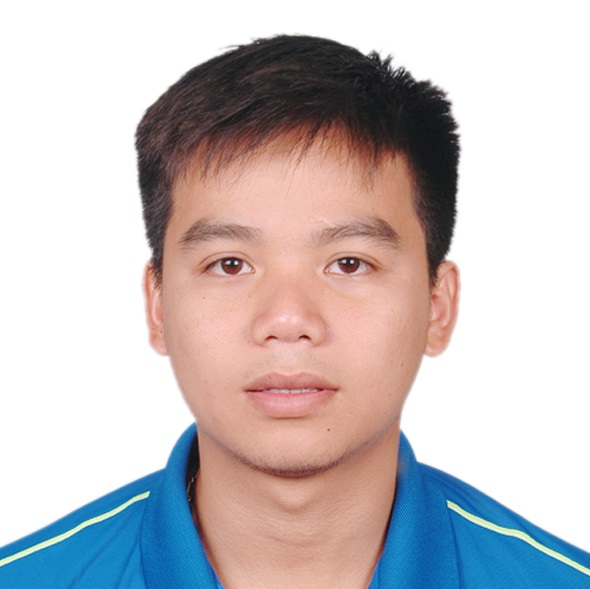
\includegraphics[scale=0.4]{hai}
\end{center}
\end{frame}

%\pagenumbering{num_style}

%\begin{frame}
%\frametitle{Overview} % Table of contents slide, comment this block out to remove it
%\tableofcontents % Throughout your presentation, if you choose to use \section{} and \subsection{} commands, these will automatically be printed on this slide as an overview of your presentation
%\end{frame}

%\begin{frame}
%  \titlepage
%\end{frame}

\section{Introduction}

%\begin{frame}{Outline}
	\begin{itemize}
		\item Introduction
		\item The first main result: correlation extraction construction 
		\item Comparison to prior work
		\item The second main result: bound on the maximum resilience
		\item The key technical idea
		\begin{itemize}
			\item Extracting one OLE over a large field
			\item Embedding multiple OLEs into an OLE over an extension field
		\end{itemize}
		\item Simple partition number
		\item Conclusions and open problems
	\end{itemize}
\end{frame}

\section{Introduction}\label{sec:intro}


\subsection{Correlation Extractors and Security Model}
\subsection{Our Contribution}


\begin{table}
\begin{center}
{\renewcommand{\arraystretch}{2.5}
\onslide<2> {}
%\onslide<3-> {}
\begin{tabular}{|>{\centering\arraybackslash} m{1.7cm} | >{\centering\arraybackslash} m{1.9cm} | >{\centering\arraybackslash} m{1.5cm} | >{\centering\arraybackslash} m{1.5cm} | >{\centering\arraybackslash} m{1.0cm} | >{\centering\arraybackslash} m{1.0cm} |}\hline 
%	{| c | c | c | c | c | c |} \hline 

Paper & Correlation  &  $m$ & $t$ & $\eps$ & \# \\\hline
%%%
\cite{FOCS:IKOS09} & \ROT[n/2] & $\alpha n$ & $\beta n$ & $2^{-\gamma n}$ & 4\\\hline
%%%
%\pause 
\multirow{2}{*}{\cite{C:GIMS15}} & \ROT[n/2] & $ \dfrac{n}{\poly\log n}$ & $(\nicefrac14 - g) n$ & $2^{-g n/m}$ & 2 \\\cline{2-6}
%%%
\ifnum\slideno>1
& \IP[\GF{2}^{n}] & $1$ & $(\nicefrac12 - g) n$ & $2^{-gn}$ & 2 \\
\hline
%%%
%\pause
%\ifnum\slideno>2 
%Our Work & \ROLE[\GF{2^n}] & $n^{1-o(1)}$ & $(\nicefrac12 - g) n$ & $2^{-gn}$ & 2\\\hline 
\textcolor{red}{Our Work} & \textcolor{red}{\IP[\bbF^{n/\log\abs\bbF}]} & \textcolor{red}{$n^{1-o(1)}$} & \textcolor{red}{$(\nicefrac12 - g) n$} & \textcolor{red}{$2^{-gn}$} & \textcolor{red}{2}\\\hline 
\fi %\fi
\end{tabular}}
%\end{tabular}
\end{center}
%\caption{
%  A qualitative summary of prior relevant works in correlation extractors and a comparison to our correlation extractor construction. 
%  All correlations have been normalized so that each party gets an $n$-bit secret share. 
%  The positive constants $\alpha,\beta,$ and $\gamma$ are minuscule. 
%  And $g<1/2$ is an arbitrary positive constant. 
%}
\label{fig:results} 
\end{table}
\subsection{Prior Related Work}\label{sec:prior}
\textcolor{red}{Talk about IKOS and GIMS here. Also talk about results related to extractors. In each other section, also include prior work discussions related to the technical contributions of each work.}
\subsection{Technical Overview}\label{sec:overview}
In \figureref{paradigm}, we present the primary technical idea underlying the constructions of our correlation extractors,  which is also common to the protocols in \cite{ISIT:IMSW14,C:GIMS15}.

%%%
\begin{figure}[htp]%\footnotesize
\begin{boxedalgo}
\begin{enumerate}[leftmargin=5mm]
	\item Clients A and B have secret shares $r_A, r_B $ respectively from a correlation from the preprocessing step\\
	\hrule
	
	\item From an ensemble of pair of linear codes $\left\{(C_i,D_i)\colon i\text{ in the index set}\right\}$, Client A and B agree on a pair of linear codes $(C,D)$.
	
	\item Let \cE be a linear code that contains the linear span of all the coordinate-wise products of each codeword in $C$ with each codeword in $D$, represented by $\cE \supseteq C*D$. \\
	\hrule
	
	\item Client A picks a random codeword $(u_{-\gamma},\dotsc,u_{-1},u_1,\dotsc,u_\eta)\in C$.
	
	\item Client B picks a random codeword $(r_{-\gamma},\dotsc,r_{-1},r_1,\dotsc,r_\eta)\in D$.
	
	\item Client A picks a random codeword $(v_{-\gamma},\dotsc,v_{-1},v_1,\dotsc,v_\eta)\in\cE$. \\ 
	\hrule 
	
	\item Clients A and B use their secret shares to help client B securely compute $ z $, which can be used to resconstruct $ z_i = u_i r_i + v_i $ for $ i \in \{-\gamma, \dotsc, -1 \} $ using ereasure recovery algorithm for $ \cE $.
	\hrule 
	
	\item Client A outputs $(u_i,v_i)$ and Client B outputs $(r_i,z_i)$, for each $i\in\{-\gamma,\dotsc,-1\}$ 
\end{enumerate}
\end{boxedalgo}
\caption{Round-optimal correlation extractor design paradigm based on Massey secret sharing scheme.}
\label{fig:paradigm}
\end{figure}













%Note that only steps (1) and (7) require interaction. 
%Step (1), which is equivalent to secure coin tossing, can be performed by either party because the parties are semi-honest. 
%Step (7) is a two-round protocol (\cf~\cite{EC:WolWul06}). 
%Hence, the overall protocol is a two-round protocol, if the client who sends the first message for step (7) also performs step (1). 
%If \cE admits an efficient erasure recovery algorithm and $d(\cE) > \gamma$, then client B can efficiently perform step (8). 
%Note that, for every $i\in\{-\gamma,\dotsc,-1\}$, the outputs $(u_i,v_i)$ and $(r_i,z_i)$ are correct \ROLE[\bbF] secret shares. 
%The privacy of this protocol, which also subsumes the argument that the output \ROLE[\bbF] secret shares are independent, relies on the particulars of the leakage model and the choices of the ensemble of codes \cC, \cD, and \cE. \\

Following this paradigm, the security argument for the correlation extractor reduces to the observation that, given any particular non-trivial linear test, a random codeword from a random code fools this linear test. 
Note that linear leakage is a special type of leakage, and surprisingly protecting only against all linear leakages suffices to protect against arbitrary leakage. 
Thus, protection against linear leakage is not only necessary but also sufficient. 

More concretely, let  $\gamma, \eta \in \bbN$ and consider any non-zero $S=(S_{-\gamma},\dotsc, S_{-1}, S_1, \dotsc, S_\eta) \in \bbF^{\gamma + \eta}$. 
The linear function $L_S\colon\bbF^{\gamma + \eta}\to\bbF$ is defined by $L_S(x) = \sum_{i \in [-\gamma,\eta]} S_ix_i$ for $x \in \bbF^s$, where $[-\gamma, \eta] = \{-\gamma,\dotsc,-1,1,\dotsc,\eta\}$.
If $x$ is chosen uniformly at random from  $\bbF^{\gamma+\eta}$ then the output of $L_S(x)$ is uniformly random over \bbF, for all non-zero $S$. 
However, if $x$ is chosen uniformly at random from a vector subspace of $\bbF^{s}$, then $L_S$ is a constant function for every $S$ in the dual of this subspace.  
So, sampling $x$ from a {\em particular subspace} of $\bbF^{s}$ is unable to fool%
\footnote{
	A distribution $\cD$ over the sample space $\bbF^{\gamma+\eta}$ $\rho$-{\em fools} a linear test $L_S$ if the distribution of $L_S(x)$, where $x\drawn \cD$, is $\rho$-close to the uniform distribution over \bbF. 
}
every linear test.
Sampling $x$ from an {\em ensemble} of subspaces of $\bbF^{s}$, on the other hand, can fool every non-trivial linear test, except with an exponentially low probability. 
Such ensembles are called a {\em family of small-bias distributions.} 
Thererfore, the privacy of client A and client B, respectively, reduces to demonstrating that the ensemble of the codes $\{C_i\}$ and the ensemble of the codes $\{D_i\}$ satisfy this property.  
We emphasize that if there exists $S$ such that the linear test $L_S$ is, say, not fooled by the ensemble of codes $\{C_i\}$ then an adversarial client B can perform a 1-bit leakage to violate the privacy of client A. \\


\noindent\textbf{Instantiation for \cite{ISIT:IMSW14,C:GIMS15}.} 
These recent works on round-optimal correlation extractor construction create the ensemble of codes as follows. 
Let $\{C_i\}$ be the set of all linear codes, and $D_i$ is the dual code of $C_i$. 
Consequently, for any pair of linear codes $(C,D)$ in the ensemble, set $\cE$ as the linear code such that the sum of every element in the codeword is 0, referred to as the {\em parity code}. Since the parity code has distance 2 and it can efficiently recover one erasure, we have $\gamma=1$. 
%We emphasize that \cite{ISIT:IMSW14,C:GIMS15} use $\bbF=\GF{2}$, while \cite{C:BloMajNgu17} uses large fields with characteristic 2. 


%Moreover, intuitively, as the probability of fooling linear tests gets closer to 1, the protocol can have higher production (if permitted by the distance of \cE) and tolerate more leakage. \cmmt{I know that here you are referring to the expression in unpredictability lemma, but its hard to understand. We should rephrase this; I don't know how though.}

%In the terminology of leakage resilience,  
%\TODO{This approach does not give high production.} \dg{But, note that in above constructions, $d(\cE) = 2$ and hence, we can do only one erasure recovery. This implies that the above small-bias distributions cannot produce high production directly. \textsc{Add a footnote on how GIMS gets more than one OT.}} 

The approach mentioned above (where $D_k$ is the dual code of $C_k$) only achieves $d(\cE)=2$ and, consequently, $\gamma=1$. 
To achieve linear production, a potential approach is to ensure that $d(\cE)$ is linear.
%
%The discussion above reduces the goals of our work to the following. 
This approach reduces the goals of our work to the following. 
\begin{boxedalgo}
	\noindent{\bfseries Our Target Properties.} 
	Over suitably chosen finite fields
	\begin{enumerate}
		\item Construct the ensemble $\{(C_i,D_i)\}$ such that the linear code $\cE\supseteq C_i*D_i$ supports $\gamma$-erasure recovery for each $i$, and 
		\item The ensembles of codes $\{C_i\}$ and $\{D_i\}$ are both families of small bias distributions. 
	\end{enumerate}
\end{boxedalgo} 

\noindent\textbf{Related work of \cite{TCC:MeiPrzWul07,ICALP:PrzWul08} using secret-sharing schemes of \cite{C:CheCra06}.}%
\footnote{
	We emphasize that the original constructions of \cite{TCC:MeiPrzWul07,ICALP:PrzWul08} used Reed-Solomon codes over large fields. 
	We believe that near-MDS AG codes (\ie, the Singleton Bound $d\leq n-k+1$ is satisfied with a small multiplicative slack) over constant size fields can also be used in their protocols.  
} 
Using Algebraic Geometry (AG) Codes, there are near-MDS codes%
\footnote{
	A maximum distance separable code, or MDS code, satisfies the Singleton Bound tightly $d= n-k+1$. 
	A near-MDS code roughly achieves this bound with a slight multiplicative slack. 
}
with one of the properties mentioned above, namely, target property (1). 
%There are Algebraic Geometry Code, which are near-MDS, with target property (1). 
There is an appropriate AG Code $C^*$ such that, if $C=D=C^*$ then the code \cE has linear distance. 
We have already discussed that any single code cannot fool all linear tests, so this idea clearly {\em does not} suffice for our goals. 
However, \cite{TCC:MeiPrzWul07,ICALP:PrzWul08} use this idea to achieve the partial goal of protection against the leakage of individual bits of the secret shares. 
In fact, the construction is robust to linear tests $S$ with small support, and there are 1-bit linear leakages with a large support that render this construction insecure. 
To achieve our goals, {we need to fool every linear test}, including the ones with large support.  %\dg{It does not fool large linear tests.}
%\TODO{Generalization from probing to arbitrary leakage.} 
\\

\noindent\textbf{Related work of \cite{FOCS:IKOS09}.} 
The approach of Ishai~\etal~\cite{FOCS:IKOS09}, which also uses this AG Code $C^*$, can be interpreted in the paradigm presented in \figureref{paradigm}, albeit a minor modification. 
The ensemble of codes $\{C_i\}$ is {\em non-linear} code,% 
\footnote{
	Concatenation of an AG code with a binary representation of the field elements, a majority encoding of each bit, and a randomized encoding for a suitable constant-size functionality. 
	The ensemble is constructed by enumerating all outcomes of the probabilistic encoding procedures.  
}
that is a family of small biased distribution, while the code $D$ is an appropriate fixed linear code. 
%The code \cE is not defined by a coordinate-wise product of the each pair of codewords in \cC and \cD, but by coordinate-wise applying a suitable (constant-size) functionality. 
%Moreover, most crucially, their approach only achieves security against one client. 
This approach, therefore, achieves security for client A against an adversarial client B. 
Recall that this is the primary reason that their construction is not round optimal. 
To achieve our goals, {we need to construct $\{(C_i, D_i)\}$ such that both $\{C_i\}$ and $\{D_i\}$ are families of small bias distributions.}  

\begin{frame}{Prior Work \& Our Contributions}
	\begin{table}
\begin{center}
{\renewcommand{\arraystretch}{2.5}
\onslide<2> {}
%\onslide<3-> {}
\begin{tabular}{|>{\centering\arraybackslash} m{1.7cm} | >{\centering\arraybackslash} m{1.9cm} | >{\centering\arraybackslash} m{1.5cm} | >{\centering\arraybackslash} m{1.5cm} | >{\centering\arraybackslash} m{1.0cm} | >{\centering\arraybackslash} m{1.0cm} |}\hline 
%	{| c | c | c | c | c | c |} \hline 

Paper & Correlation  &  $m$ & $t$ & $\eps$ & \# \\\hline
%%%
\cite{FOCS:IKOS09} & \ROT[n/2] & $\alpha n$ & $\beta n$ & $2^{-\gamma n}$ & 4\\\hline
%%%
%\pause 
\multirow{2}{*}{\cite{C:GIMS15}} & \ROT[n/2] & $ \dfrac{n}{\poly\log n}$ & $(\nicefrac14 - g) n$ & $2^{-g n/m}$ & 2 \\\cline{2-6}
%%%
\ifnum\slideno>1
& \IP[\GF{2}^{n}] & $1$ & $(\nicefrac12 - g) n$ & $2^{-gn}$ & 2 \\
\hline
%%%
%\pause
%\ifnum\slideno>2 
%Our Work & \ROLE[\GF{2^n}] & $n^{1-o(1)}$ & $(\nicefrac12 - g) n$ & $2^{-gn}$ & 2\\\hline 
\textcolor{red}{Our Work} & \textcolor{red}{\IP[\bbF^{n/\log\abs\bbF}]} & \textcolor{red}{$n^{1-o(1)}$} & \textcolor{red}{$(\nicefrac12 - g) n$} & \textcolor{red}{$2^{-gn}$} & \textcolor{red}{2}\\\hline 
\fi %\fi
\end{tabular}}
%\end{tabular}
\end{center}
%\caption{
%  A qualitative summary of prior relevant works in correlation extractors and a comparison to our correlation extractor construction. 
%  All correlations have been normalized so that each party gets an $n$-bit secret share. 
%  The positive constants $\alpha,\beta,$ and $\gamma$ are minuscule. 
%  And $g<1/2$ is an arbitrary positive constant. 
%}
\label{fig:results} 
\end{table}
\end{frame}

\begin{frame}{Main Result I}
	\begin{theorem}
	[High Resilience, High Production CorrExt]
	\label{thm:construction}
	For all constants $0<\delta<1/2$
	\begin{itemize}
		\item $ \exists $ a correlation $(R_A,R_B)$, and
		\item $ \exists $ a two-round $(n,m = n^{1-o(1)},t,\eps)$-CorrExt for $(R_A,R_B)$
	\end{itemize}
	such that 
	\begin{itemize}
		\item if $t=(\nicefrac12-g)n$ then $\eps=2^{-(g-\delta)n/2}$.
	\end{itemize} 
	\end{theorem}
	\pause
	{\setbeamercolor{block title}{bg=purple, fg=white}
	\begin{block}{Questions}
		\begin{itemize}
		\item Does there exist a CorrExt for $ \IP[\bbF^n] $ that can achieves over $ \nicefrac{1}{2} $ fractional leakage resilience? \pause
		\item More generally, can we meaningfully \underline{upper-bound} the maximum leakage resilience of any correlation? 
		\end{itemize}
	\end{block}
	}
\end{frame}

\begin{frame}{Main Result II}
	\begin{theorem}[Hardness of Correlation Extraction]
	\label{thm:hardness} 
	Let $(\bbF,+,\cdot)$ be an arbitrary field.
	\begin{itemize}
		\item $ \exists $ a universal constant $\eps^*>0$
	\end{itemize}
	such that
	\begin{itemize}
		\item  for $(R_A,R_B)=\IP [\bbF^k] $, %or $(R_A,R_B)=\ROLE[\GF{2^{n/2}}]$, 
		\item any $(n,1,%(n/k)\ceil{(k+1)/2}
		n/2,\eps)$-CorrExt for $(R_A,R_B)$ has $\eps\geq\eps^*$, where $n=k\log\abs\bbF$.  
	\end{itemize}
\end{theorem}

{\setbeamercolor{block title}{bg=Gray, fg=white}
\begin{block}{Note}
	This result proves the \underline{optimality} of the leakage resilience achieved by our extractor.
\end{block}}

\end{frame}

\section{Main Technical Contributions}
\begin{frame}{CorrExt Construction Overview I}
%	\begin{itemize}
%		\item $ \IP[\bbK]^{[t]} \rightarrow \ROLE[\bbK] \rightarrow \OLE[\bbK]$, where $ \bbK = \GF{2^{\delta n}} $
%		\item Simultaneously embed $ \OLE[\GF 2]^m $ into one $ \OLE[\bbK] $
%		\item This embedding relies on finding solutions to a new combinatorial problem
%		
%		\TODO{draw a picture}
%	\end{itemize}
	A natural generalization of \OT:
	\begin{definition}[Oblivious Linear-Function Evaluation (\OLE)]
		An oblivious linear-function evaluation over a field $ \bbF $
		\begin{itemize}
			\item represented as $ \OLE[\bbF] $
			\item takes $ (A,B) \in \bbF^2 $ from Alice, and $ X \in \bbF $ from Bob
			\item provides $ Z = AX +B $ to Bob 
		\end{itemize}  
	\end{definition}
	\pause
	{\setbeamercolor{block title}{bg=Gray, fg=white}
	\begin{block}{Notes}
	\begin{itemize}
		\item Alice gains no additional advantage in predicting $ X $
		\item Bob gains no additional advantage in predicting  $ A $
		\item  \OT is functionally equivalent $ \OLE[\GF{2}] $ since $ x_b = (x_1 - x_0)b + x_0 $
		%\item Random oblivious linear-function evaluation $ (\ROLE) $ is a randomized version of $ \OLE $.
	\end{itemize}
	\end{block}}
	
\end{frame}

\begin{frame}{CorrExt Construction Overview II}
	\begin{figure}
\onslide<1->{\small Goal: Alice and Bob want to produce $m$ {\OLE}s over \GF{2}.}
\hrule
\begin{center}

\begin{adjustbox}{max width={\textwidth}}
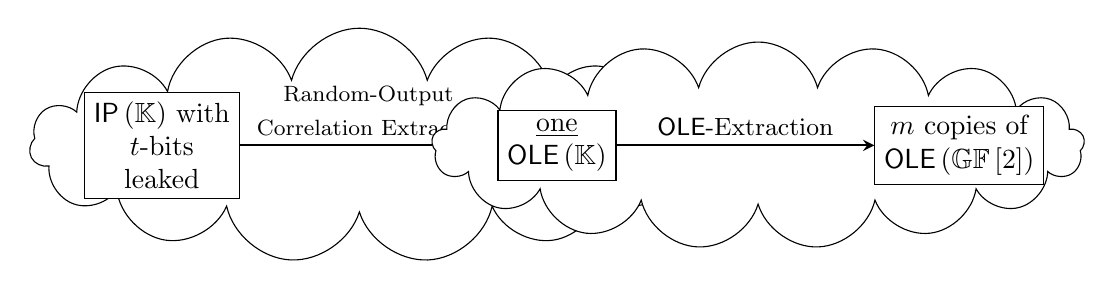
\begin{tikzpicture}[every node/.style={fill=white}, >=stealth]

%% Leaky IP
\onslide<2->{\node[draw, rectangle, align=center] (IP) {\IP[\bbK] with \\ $t$-bits\\leaked};}

%% OLE K
\onslide<3->{\node[draw, rectangle, right=.27\linewidth of IP, align=center] (OLEk) {\underline{one}\\\OLE[\bbK]};}

%% m-OLE
\onslide<4->{\node[draw, rectangle, right=.27\linewidth of OLEk, align=center] (mOLE) {$m$ copies of\\ \OLE[\GF{2}]};}

\begin{pgfonlayer}{background}

%% second arrow
\onslide<4->{\draw[thick, ->] (OLEk) -- (mOLE) node[above, midway, fill opacity=0, text opacity=1] {\footnotesize \OLE[]-Extraction};}

\onslide<5>{
%% first cloud
\node[draw, cloud, cloud ignores aspect, fit=(IP.center)(OLEk.center), cloud puffs=15, inner ysep=1.7em, inner xsep=1.2em] (cloud1) {};
}

%% first arrow
\onslide<3->{\draw[thick, ->] (IP) -- (OLEk) node[above, midway, align=center,fill opacity=0, text opacity=1] {\footnotesize Random-Output\\\footnotesize Correlation Extractor};}

\onslide<6->{
%% second cloud
\node[draw, cloud, cloud ignores aspect, fit=(OLEk.center)(mOLE.center), cloud puffs=17, inner ysep=1.5em, inner xsep=1em] (cloud2) {};

%% second arrow (again)
\draw[thick, ->] (OLEk) -- (mOLE) node[above, midway,fill opacity=0, text opacity=1] {\small \OLE[]-Extraction};
}


\end{pgfonlayer}


\end{tikzpicture}
\end{adjustbox}

\end{center}
\end{figure}
	\only<5>{Natural generalization of the \cite{C:GIMS15} protocol for \IP[] over \GF{2} to \IP[] over large fields.}
	\only<6-8>{Embed $ m $ copies of $\OLE[\GF{2}] $ into \underline{one} $ \OLE[\bbF] $, where $ \bbF $ is a large field of characteristic 2}
	\only<7>{\begin{center}
			\textcolor{red}{\Large One of Our Technical Contributions}
	\end{center}}
	\only<8>{\setbeamercolor{block title}{bg=Gray, fg=white}
		\begin{block}{Notes}
			\begin{itemize}
				\item The larger the value of $ m $, the better the production rate.
				\item This embedding relies on finding solutions to \textcolor{red}{the tri-colored sum-free sets problem}.
			\end{itemize}
		\end{block}
	}
\end{frame}

\begin{frame}{Tri-colored Sum-free Sets Problem}
	
	{\setbeamercolor{block title}{bg=ForestGreen, fg=white}
	\begin{block}{Tri-colored Sum-free Sets Problem}
		Find two ordered sets $ S = (s_1, s_2, \cdots, s_m) $ and $ T = (t_1, t_2, \cdots, t_m) $ \st
		\begin{itemize}
			\item $ s_i$ and $ t_i $ are non-negative integers for every $ i $
			\item $ s_i + t_j < n $ for every $ i, j $
			\item $ s_i + t_i \neq s_j + t_k  $ for every $ i, j, k $ that are not all identical
			\item $ m $ is maximized 
		\end{itemize} 
	\end{block}}
	\pause

	{\setbeamercolor{block title}{bg=Gray, fg=white}
	\begin{block}{Notes}
		\begin{itemize}
			\onslide<2->{\item This problem is a generalization of the \textcolor{red}{well-known 3-free set problem}\only<2>{\footnote{3-free set problem is a problem of constructing dense sets of integers that are free of arithmetic progressions of length 3}} %(sets that avoid any arithmetic progressions of length 3) problem.
			\begin{itemize}
				\item For $ s_i = t_i $, this problem is identical to the 3-free set problem 
			\end{itemize}}
			\only<3->{
			\item Using existing explicit constructions of the 3-free set, we achieve $ m = n^{1-o(1)} $
			\item In an ongoing work, we show that $m = \Theta(n)$ is impossible} 
		\end{itemize}
		
	\end{block}}

%	\pause
%	\begin{lemma}
%		Recently we show that $ m = o(n) $.
%	\end{lemma}
\end{frame}

%\begin{frame}{Our Embedding Problem}
%	\begin{itemize}
%	\item Our aim: Suppose there is an oracle that performs OLE over an extension field $ \bbK $. By making only one call to this oracle, no other communication allows, how many OLEs over the field $ \bbF $ can be calculated? %\pause
%	\item More concretely: 
%	\begin{itemize}
%		\item Given an oracle that take as input $ A, B \in \bbK  $ from Alice and $ X \in \bbK $ from Bob, and outputs $ Z = A\cdot X + B $ to Bob. %\pause
%		
%		\item  Alice: $ (a_0, a_1, \cdots, a_{m-1}) \in \bbF^m $ and $ (b_0, b_1, \cdots, b_{m-1}) \in \bbF^m $. %\pause
%		\item  Bob: $ (x_0, x_1, \cdots, x_{m-1}) \in \bbF^m $. %\pause
%		\item  We want Bob to obtain $ (z_0, z_1, \cdots, z_{m-1}) \in \bbF^m $, where $ z_i = a_i \cdot x_i + b_i $. %\pause
%		\item Intuitively, we want to maximize $ m $ and embed $ OLE(\bbF)^m $ into one $ OLE(\bbK) $ %\pause
%	\end{itemize}
%	\item Easy to embed for $ m = 1 $ but can we do better? 
%\end{itemize}
%\end{frame}
%
%\begin{frame}{Embedding}
%	\begin{itemize}
%		\item Given $ S = (s_0, s_1, \cdots, s_{m-1}) $ and $ T = (t_0, t_1, \cdots, t_{m-1}) $ to be a solution to the combinatorial problem. %\pause
%		\item $  A = \sum_{i = 0}^{m-1} a_i \zeta^{s_i} $ %\pause
%		\item $ B = \sum_{i=0}^{n-1} r_i \zeta^i $, where \\ $ r_i = \begin{cases}
%		b_k & ,\text{ if } i = s_k + t_k \text{ for some } k \in \{0, 1, \cdots, m-1\} \\
%		U_{\bbF} & ,\text{ otherwise.}
%		\end{cases} $ %\pause
%		\item $ X = \sum_{i=0}^{m-1} x_i \zeta^{t_i} $ %\pause
%		\item Invoke the oracle, Bob receives $ Z = AX + B $. %\pause
%		\item $ A X = \sum\limits_{i,j} a_i x_j \zeta^{s_i + t_j} = \sum\limits_{i} a_i x_i \zeta^{s_i + t_i} + \sum\limits_{j \neq k} a_j x_k \zeta^{s_j + t_k} $. %\pause
%		\item The coefficient of $ \zeta^{s_i + t_i} $ in $ Z $ is $ z_i = a_i x_i + b_i $ since $ s_i + t_i \neq s_j + t_k $.
%	\end{itemize}
%	
%\end{frame}

\begin{frame}{Upper-Bounding Leakage Resilience}

{\setbeamercolor{block title}{bg=Gray, fg=white}
	\begin{block}{Question}
		Which techniques can be used to upper-bound the maximum leakage resilience of a correlation?
	\end{block}
}

\pause

{\setbeamercolor{block title}{bg=Turquoise, fg=white}
	\begin{block}{Existing Approach}
		Partition argument
%		\begin{itemize}
%			\item $ n/2 $ samples of the ROT correlation cannot be resilient to more than $ n/4 $ bits of leakage
%			\item Alice emulates $ n/4 $ independent samples
%			\item Bob emulates $ n/4 $ independent samples
%			\item Reimagine any correlation extractor
%		\end{itemize}		
	\end{block}
}

\pause

{\setbeamercolor{block title}{bg=Maroon, fg=white}
\begin{block}{Bottleneck}
\begin{itemize}
	\item Applies only to ``multiple independent samples of small correlations", for instance, $ \ROT[n/2] $
	\item \textcolor{red}{Does not extend to secret shares sampled from globally correlated correlations, for example, $ \IP[\bbF^n] $}
\end{itemize}
\end{block}
}

\end{frame}

\begin{frame}{Simple Partition Number (Our Technical Contribution)}
	\begin{definition}[Simple Graph]
		A \textit{simple graph} is a bipartite graph such that each of its
		connected component is a biclique (complete bipartite graph)
	\end{definition}
	\pause
	\begin{definition}[Simple Partition Number]
		The \textit{simple partition number} of a bipartite graph $G$, represented
		by $\sp G$, is the minimum number of simple graphs needed to
		partition its edges.
	\end{definition}
	\pause
	\begin{figure}[htb] \footnotesize
\begin{center}
\begin{tikzpicture}[
  vert/.style = {node distance = 5mm, circle, draw, fill = purdue-gold!40, thick, inner sep = 1pt},  
  bdd/.style = {rectangle, draw, inner sep = 5mm}, 
                   ]

%%% First Correlation 
\node [vert] (a00) at (0,0) {00}; 
\node [vert, below = of a00] (a01) {01}; 
\node [vert, below = of a01] (a10) {10}; 
\node [vert, below = of a10] (a11) {11}; 

\node [vert, node distance = 10mm, right = of a00] (b00) {00}; 
\node [vert, below = of b00] (b01) {01}; 
\node [vert, below = of b01] (b10) {10}; 
\node [vert, below = of b10] (b11) {11}; 


\draw [thick] (a00) -- (b00)  (a00) -- (b01)  (a00) -- (b10)  (a00) -- (b11); 
\draw [thick] (a01) -- (b00)  (a01) -- (b10); 
\draw [thick] (a10) -- (b00)  (a10) -- (b01); 
\draw [thick] (a11) -- (b00)  (a11) -- (b11); 

%\pause 

\node at (2.3,-1.7) {=}; 

\node [vert] (c00) at (3,0) {00}; 
\node [vert, below = of c00] (c01) {01}; 
\node [vert, below = of c01] (c10) {10}; 
\node [vert, below = of c10] (c11) {11}; 

\node [vert, node distance = 10mm, right = of c00] (d00) {00}; 
\node [vert, below = of d00] (d01) {01}; 
\node [vert, below = of d01] (d10) {10}; 
\node [vert, below = of d10] (d11) {11};

\draw[draw=red!70!black, thick] (c00) -- (d00)  (c00) -- (d11);
\draw[draw=blue!70!black, thick] (c01) -- (d10);
\draw[draw=green!70!black, thick] (c10) -- (d01);
\draw[draw=red!70!black, thick] (c11) -- (d00)  (c11) -- (d11);


\node at (5.3, -1.7) {+};

\node [vert] (e00) at (6,0) {00}; 
\node [vert, below = of e00] (e01) {01}; 
\node [vert, below = of e01] (e10) {10}; 
\node [vert, below = of e10] (e11) {11}; 

\node [vert, node distance = 10mm, right = of e00] (f00) {00}; 
\node [vert, below = of f00] (f01) {01}; 
\node [vert, below = of f01] (f10) {10}; 
\node [vert, below = of f10] (f11) {11};

\draw[draw=red!70!black, thick] (e00) -- (f01)  (e00) -- (f10);
\draw[draw=green!70!black, thick] (e01) -- (f00);
\draw[draw=green!70!black, thick] (e10) -- (f00);


\end{tikzpicture}
\end{center}
%\caption{A decomposition of $ \IP {} $ into 2 simple graphs.}
\label{fig:IP^2-sp-decomp}
\end{figure}





\end{frame}
\begin{frame}{Graph Representation of Correlations}
	\begin{definition}[Graph of a Correlation]
		A weighted bipartite graph $  G = (L, R, E) $
		\begin{itemize}
	  		\item $ L $: the set of all possible private shares $ r_A $ for Alice
	  		\item $ R $: the set of all possible private shares $ r_B $ for Bob
			\item Weight of the edge $ (r_A, r_B) $ is  $ p(r_A, r_B) $
		\end{itemize}
	\end{definition}
	\begin{figure}[htp] \footnotesize
\begin{center}
\begin{tikzpicture}[
vert/.style = {node distance = 5mm, circle, draw, fill = purdue-gold!40, thick, inner sep = 1pt},  
bdd/.style = {rectangle, draw, inner sep = 5mm}, 
cc/.style = {rounded corners = 5pt, fill = black!50, pattern = crosshatch dots, pattern color = gray}, 
minimum size = 5mm,
]
%[
%vert/.style = {node distance = 5mm, circle, draw, fill = black!10, thick, inner sep = 1pt},  
%bdd/.style = {rectangle, draw, inner sep = 5mm}, 
%cc/.style = {rounded corners = 5pt, fill = black!50, pattern = crosshatch dots, pattern color = gray}, 
%minimum size = 5mm,
%]

%%% 
\node at (0,0) (l1) {L};
\node [vert, below = of l1] (c00)  {}; 
\node [vert, below = of c00] (c01) {$r_A$}; 
\node [vert, below = of c01] (c10) {}; 
%\node [vert, below = of c10] (c11) {11}; 

\node [node distance = 15mm, right = of l1] (r1) {R};
\node [vert, below = of r1] (d00) {}; 
\node [vert, below = of d00] (d01) {$ r_B $}; 
\node [vert, below = of d01] (d10) {}; 
%\node [vert, below = of d10] (d11) {11};

\draw [thick] (c01) -- (d01) node [midway, above] {$ p(r_A, r_B) $};

\coordinate (temp) at ($0.5*(c10)+0.5*(d10)$);
\node[node distance = 1 cm, below of = temp] {\underline{Graph of General Correlation}}; 

%\pause 

%%% ROT
%\node [node distance = 1cm, right = of r1] (l2) {$ (x_0, x_1) $};
%\node [vert, below = of l2] (a00) {00}; 
%\node [vert, below = of a00] (a01) {01}; 
%\node [vert, below = of a01] (a10) {10}; 
%\node [vert, below = of a10] (a11) {11}; 
%
%\node [right = of l2] (r2) {$(b, x_b)$};
%\node [vert, below = of r2] (b00) {00}; 
%\node [vert, below = of b00] (b01) {01}; 
%\node [vert, below = of b01] (b10) {10}; 
%\node [vert, below = of b10] (b11) {11}; 
%
%\draw (a00) -- (b00) (a00) -- (b10); 
%\draw (a01) -- (b00) (a01) -- (b11); 
%\draw (a10) -- (b01) (a10) -- (b10); 
%\draw (a11) -- (b01) (a11) -- (b11); 
%
%\coordinate (temp) at ($0.5*(a11)+0.5*(b11)$);
%\node[below of = temp] {\underline{Random Oblivious Transfer}}; 

%\pause 

%% IP
%%% First Correlation 
%\node [node distance = 3cm, right = of r1] {$ \pred{IP} $};

\node [vert, node distance = 3cm, right = of b00] (e00) {00}; 
\node [vert, below = of e00] (e01) {01}; 
\node [vert, below = of e01] (e10) {10}; 
\node [vert, below = of e10] (e11) {11}; 

\node [vert, node distance = 15mm, right = of e00] (f00) {00}; 
\node [vert, below = of f00] (f01) {01}; 
\node [vert, below = of f01] (f10) {10}; 
\node [vert, below = of f10] (f11) {11}; 


\draw [thick] (e00) -- (f00)  (e00) -- (f01)  (e00) -- (f10)  (e00) -- (f11); 
\draw [thick] (e01) -- (f00)  (e01) -- (f10); 
\draw [thick] (e10) -- (f00)  (e10) -- (f01); 
\draw [thick] (e11) -- (f00)  (e11) -- (f11);

\coordinate (temp) at ($0.5*(e11)+0.5*(f11)$);
\node[below of = temp, align=center] {\underline{$ \IP[\GF{2}^2] $}}; 


\end{tikzpicture}
%\caption{Some representative examples of a correlation}
\end{center}
\end{figure}

\end{frame}

\begin{frame}{Connection between Maximum Leakage and Simple Partition Number}
	\begin{lemma}[Connecting Max. Resilience to $\sp G $]
		\begin{itemize}
			\item Suppose $ G = (R_A, R_B) $ is a correlation 
			\item Suppose $ \exists $ $\Lambda$ simple graphs that partition the edges of the graph $ G $
			\item Then $ G $ is not resilient to $ \log \Lambda $ bits of leakage.
		\end{itemize}
		
	\end{lemma}
	\pause
	
	{\setbeamercolor{block title}{bg=Black!80, fg=white}
	\begin{block}{Intuition}
		An upper bound on the simple partition number of a correlation implies an upper bound on the maximum leakage resilience of the correlation
	\end{block}
	}

%	\begin{itemize}
%		%\item Consider $ \pi $ resilient to $ \log \Lambda $-bit leakage and securely implements one $\pred{OLE} $.
%		\item Consider the leakage $ \cL: E(G) \rightarrow [\Lambda] $ \st $ \forall e \in E(G), \cL(e) = \ell $ and $ e \in E(G^{(\ell)}) $ 
%		\item Conditioned on the leakage being $ \ell $, the correlaiton $ (R_A, R_B | \ell) \equiv G\p\ell$ is a simple correlation 
%		\item Simple correlations are useless for correlation extractor by \cite{}.
%	\end{itemize}

\end{frame}

\begin{frame}{Estimating Simple Partition Number}
	\begin{figure}
\begin{center}
%\begin{table}
{\renewcommand{\arraystretch}{2}
\begin{tabular}{|c|c|c|c|}\hline
Correlation & Secret Share & Simple Partition  & Fractional Leakage\\
Description & Size (s) & Number (\pred{sp}) & Bound ($\log\pred{sp}/s$)\\\hline 
$\ROT[n/2]$ & $n$ & $2^{n/4}$ & \begin{adjustbox}{valign=m}

\begin{tikzpicture}
	\only<1,3->{\node[] {1/4};}
	\only<2>{\node[draw, red, circle, ultra thick, inner sep=2pt] {\textcolor{black}{1/4}};}
\end{tikzpicture}
\end{adjustbox} \\\hline 
%$\ROLE[\bbF]^{n/2}$ & $n\log\abs\bbF$ & $\abs{\bbF}^{n/4}$ & $1/4$\\\hline
$\IP[\bbF^n]$ & $n\log\abs\bbF$ & $\abs{\bbF}^{n/2}$ & $1/2$\\\hline 
\end{tabular}
%\begin{tabular}{| c | c | c | c | c | c |}\hline 
%& Correlation & Number of \OT{}s  & Number of & Simulation  & Round\\
%& Description  & Produced $(m)$ & Leakage bits $(t)$ & Error $(\eps)$ & Complexity \\\hline
%\cite{FOCS:IKOS09} & \ROT[n/2] & $\alpha n$ & $\beta n$ & $2^{-\gamma n}$ & 4\\\hline
%\multirow{2}{*}{\cite{C:GIMS15}} & \ROT[n/2] & $n/\poly\log n$ & $(\nicefrac14 - g) n$ & $2^{-g n/m}$ & 2 \\\cline{2-6} 
%& \IP[\GF{2}^{n}] & $1$ & $(\nicefrac12 - g) n$ & $2^{-gn}$ & 2\\
%\hline\hline
%%Our Work & \ROLE[\GF{2^n}] & $n^{1-o(1)}$ & $(\nicefrac12 - g) n$ & $2^{-gn}$ & 2\\\hline 
%Our Work & \IP[\bbF^{n/\log\abs\bbF}] & $n^{1-o(1)}$ & $(\nicefrac12 - g) n$ & $2^{-gn}$ & 2\\\hline 
%\end{tabular}
%\end{tabular}
}
\end{center}
%\caption{
%  A summary of the estimates of the simple partition number for the correlations relevant to our work.   
%}
\label{fig:sp} 
\end{figure}







	{\setbeamercolor{block title}{bg=Gray, fg=white}
		\only<2>{\begin{center}\textcolor{red}{\Large Subsumes the partition argument}\end{center}}
		\begin{block}{Note}
			\begin{itemize}
				%\item $ s $ is the secret share size
				\item $ (\log \pred{sp})/s $ is the upper bound on the maximum fractional leakage resilience
			\end{itemize}
		\end{block}
	}
%	\begin{lemma}
%		$ \sp{\IP ({\bbF^n})} \leq \abs{\bbF} ^{\ceil{(n+1)/2}}$
%	\end{lemma}
\end{frame}

%\begin{frame}{Relevant Prior Work on Common Information}
%
%	{\setbeamercolor{block title}{bg=red, fg=white}
%	\begin{block}{Mutual information $ I(R_A, R_B) $}
%		\begin{itemize}
%			\item $ \# $ bits of the secret key that two parties can agree on
%		\end{itemize}
%	\end{block}}
%	\pause
%	{\setbeamercolor{block title}{bg=brown, fg=white}
%	\begin{block}{\gacs-\korner \cite{} common information  $ K(R_A, R_B) $}
%		\begin{itemize}
%			\item The largest entropy of the common random variable that each party can generate based on their respective secret share
%			\item Corresponding to \textit{number of connected components}
%		\end{itemize}
%	\end{block}}
%	\pause
%	{\setbeamercolor{block title}{bg=blue, fg=white}
%	\begin{block}{Wyner's common information \cite{} $ J(R_A, R_B) $}
%		\begin{itemize}
%			\item Min. amount of leakage that kills the possibility of key agreement
%			\item Corresponding to \textit{biclique partition number}
%		\end{itemize}
%	\end{block}}
%\end{frame}



\begin{frame}{Conclusions and Open Problems}

	{\setbeamercolor{block title}{bg=brown, fg=white}
	\begin{block}{Conclusions}
		\begin{itemize}
			\item $ \exists $ a correlation that  
			\begin{itemize}
				\item generates $ n $-bits secret shares
				\item  produces $ n^{1-o(1)} $ secure $\OT$s
				\item resiliences to $ n/2 $-bits of leakage 
			\end{itemize}
			\item Introduces a graph-theoretic measure 
			\begin{itemize}
				\item to upper-bound the leakage resilience of correlations
				\item the simple partition number $ \pred{sp} $ 
			\end{itemize}
		\end{itemize}
	\end{block}
	}
	\pause

	{\setbeamercolor{block title}{bg=Green, fg=white}
	\begin{block}{Open Problems}
		\begin{itemize}
			\item Can we break the barrier of 1/2 fractional leakage?
			\item Asymptotic and concrete constructions for our combinatorial problem
			\item Algorithmic techniques to explore the hardness, estimate, and approximate $ \pred{sp} $ of general correlations
		\end{itemize}		
	\end{block}
	}
\end{frame}

\bibliographystyle{alpha}
\bibliography{math,crypto}
\end{document}
